\section{Thiết kế hệ thống phần mềm và kiến trúc vận hành tổng thể}

\subsection{Tổng quan kiến trúc hệ thống}

Hệ thống được xây dựng như một ứng dụng web nguyên khối nhẹ trên nền Flask. Lựa chọn này nhằm giảm số lượng thành phần phải triển khai, giữ chi phí vận hành ở mức thấp và tập trung nỗ lực phát triển vào mối liên hệ giữa giao diện, logic nghiệp vụ và mô hình học máy. Về bản chất, kiến trúc hiện tại mang đặc trưng của một \textit{modular monolith}: toàn bộ thành phần cùng chạy trong một tiến trình ứng dụng, nhưng vẫn được phân tách thành các mô-đun theo chức năng.

Nếu nhìn theo quan điểm MVC mở rộng, kiến trúc có thể được mô tả qua bốn lớp chính. Lớp \textit{view} gồm các template trong \texttt{app/templates}. Lớp \textit{controller} gồm các route Flask và các mô-đun điều phối trong \path{app/controllers}. Lớp \textit{model} tập trung ở \texttt{PhonePriceModel} cùng các tiện ích dữ liệu liên quan. Cuối cùng là lớp cấu hình và dữ liệu, bao gồm settings, credentials, catalog thiết bị, CSV dataset, JSON state và các model pickle.

\begin{figure}[H]
    \centering
    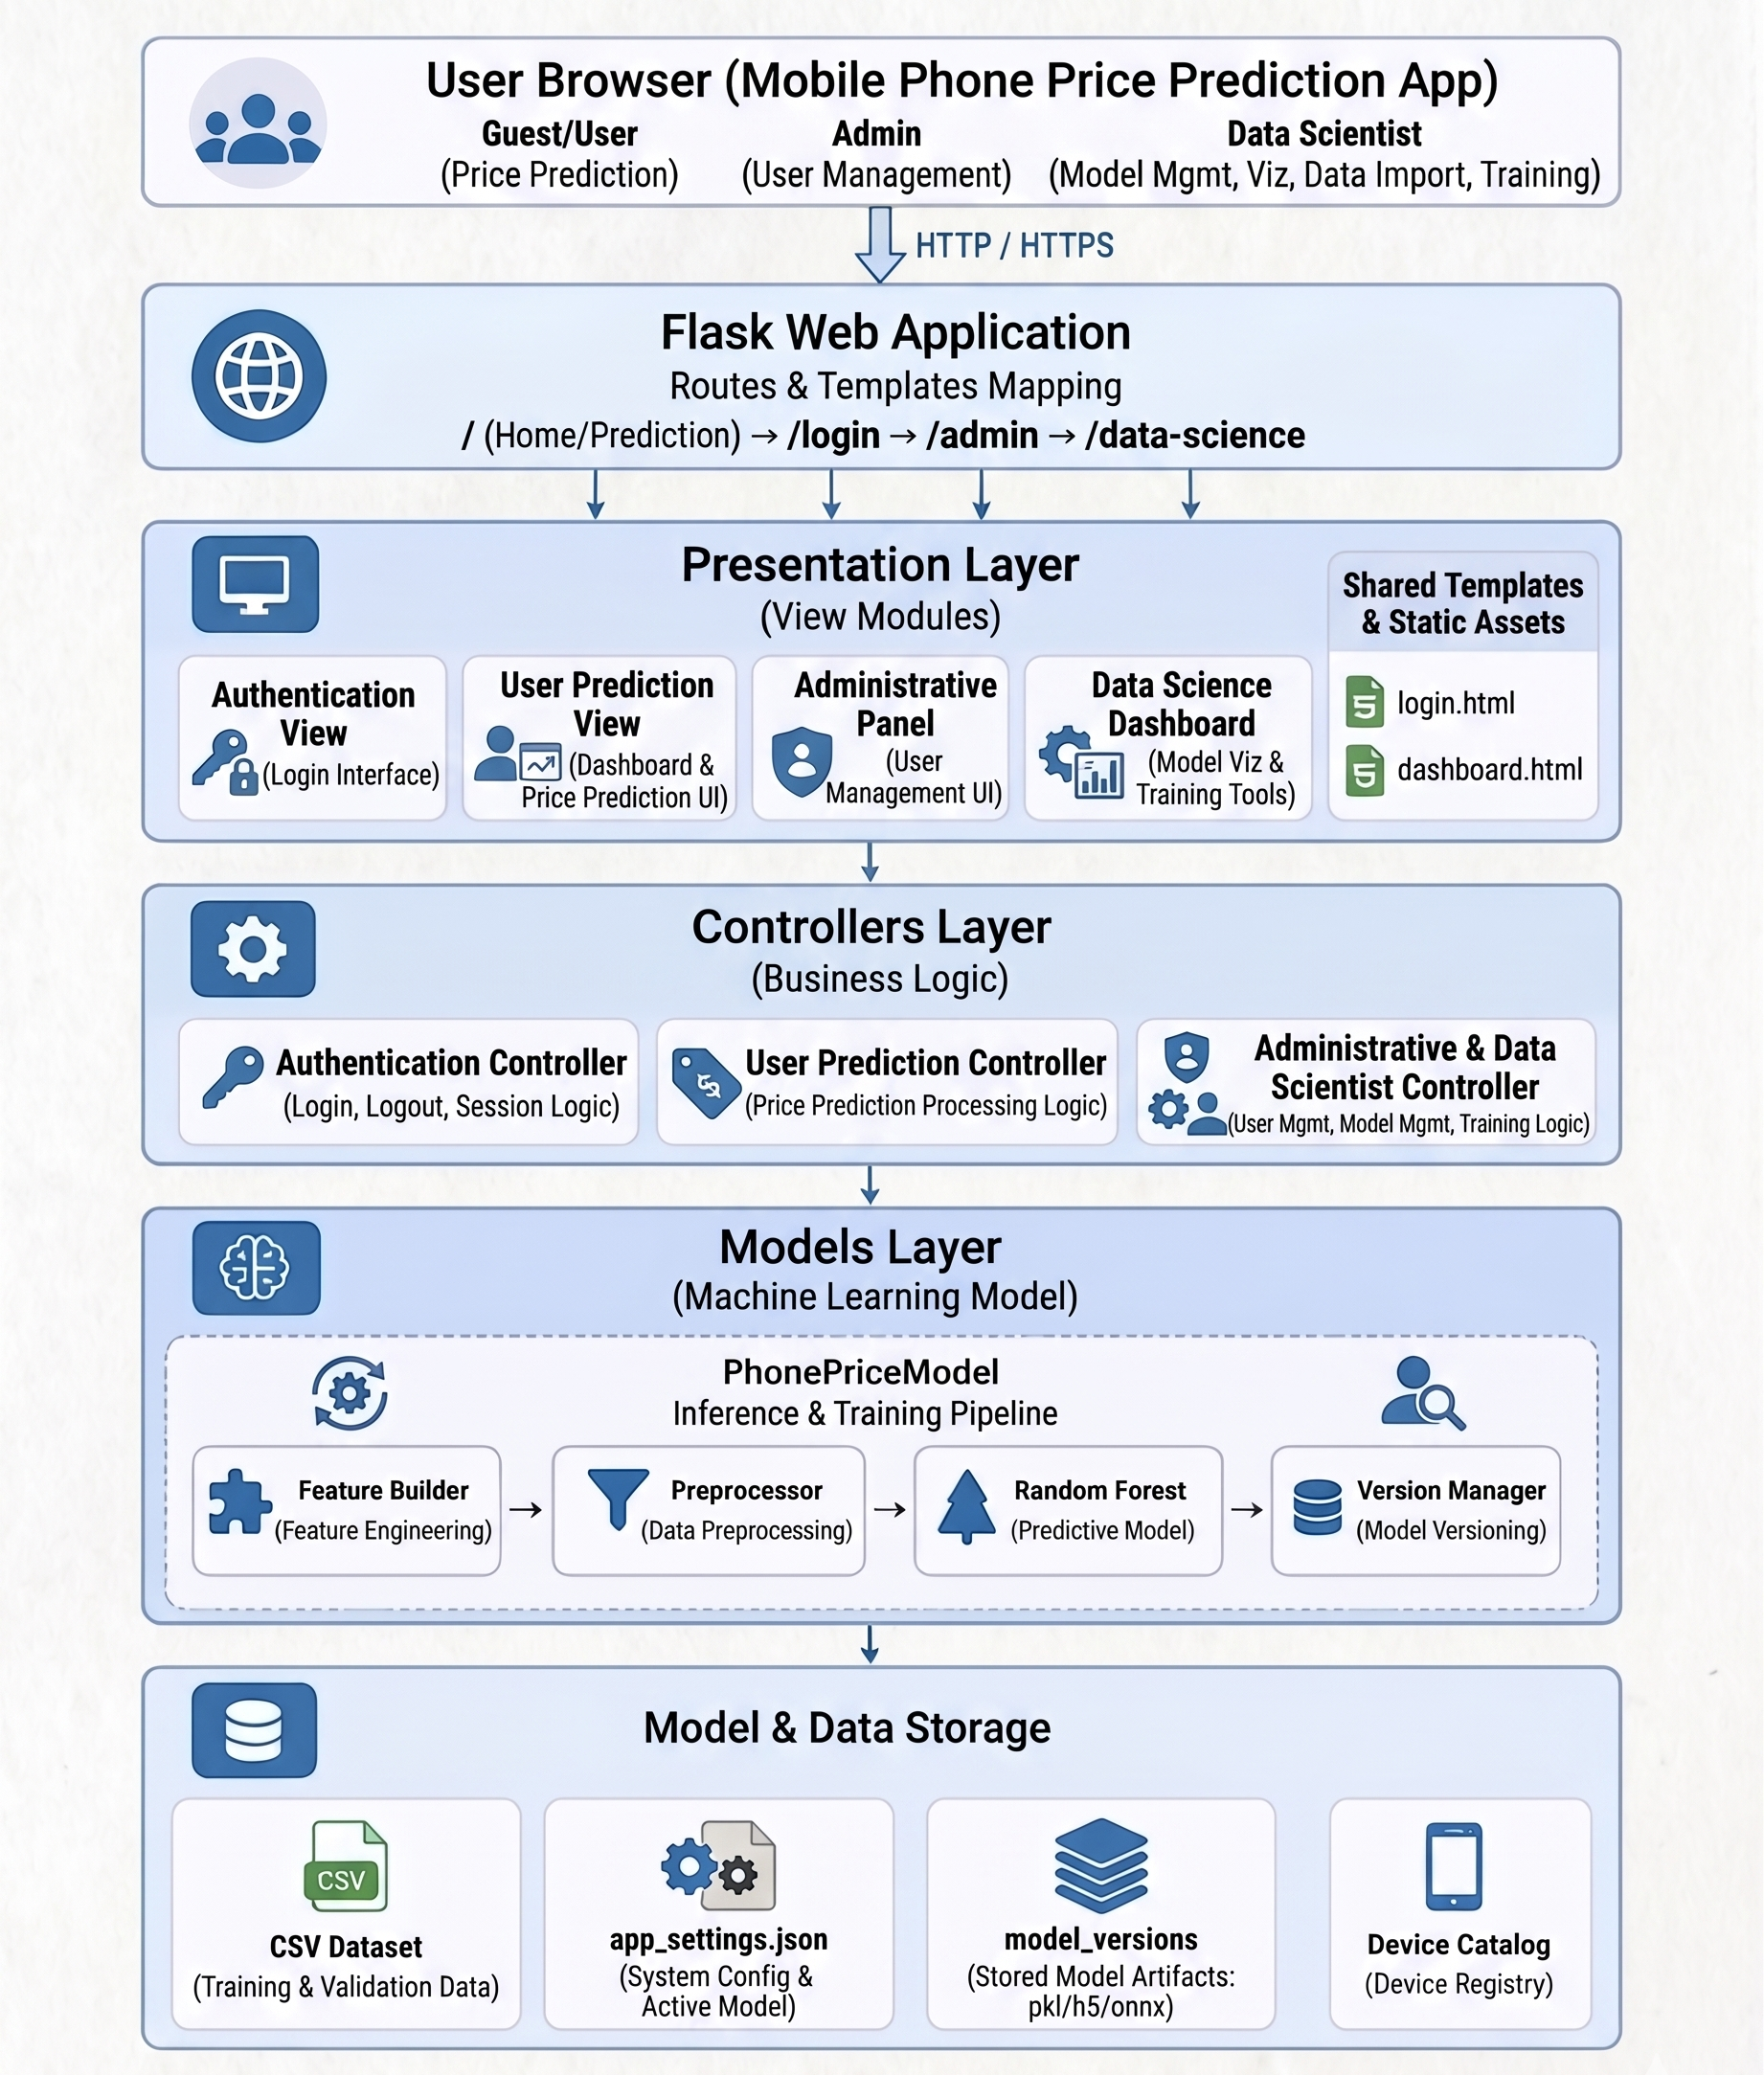
\includegraphics[width=0.9\textwidth]{graphics/system_architecture.png}
    \caption{Sơ đồ kiến trúc tổng thể của hệ thống}
    \label{fig:system-architecture}
\end{figure}

\begin{itemize}
    \item \textbf{View Layer:} Lớp giao diện gồm các template hiển thị cho người dùng, tiêu biểu như \path{app/templates/login.html} và \path{app/templates/dashboard.html}. Trong đó, \path{dashboard.html} được sử dụng như một template dùng chung cho cả Admin và Data Scientist. Nội dung hiển thị được điều chỉnh động theo role và theo section đang được truy cập, nhờ đó lớp giao diện vẫn bảo đảm được sự tách bạch về mặt trình diễn mà không cần tách thành quá nhiều file template riêng.

    \item \textbf{Controller Layer:} Lớp điều phối bao gồm hai nhóm thành phần chính: cơ chế định tuyến và kiểm soát quyền truy cập trong \path{app/app.py}, cùng với các mô-đun nghiệp vụ trong thư mục \path{app/controllers}. Cụ thể, \path{app/app.py} đảm nhiệm việc định tuyến request, kiểm tra session role và điều phối người dùng đến đúng chức năng tương ứng. Trong nhóm controller chuyên biệt, \path{app/controllers/auth_controller.py} xử lý xác thực và thông tin người dùng, \path{app/controllers/admin_controller.py} phụ trách logic quản lý model, dataset, visualization và các thao tác CRUD người dùng, trong khi \path{app/controllers/user_controller.py} đảm nhiệm logic dự đoán giá.

    \item \textbf{Model Layer:} Lớp mô hình tập trung vào thành phần học máy và các tiện ích dữ liệu đi kèm, với hạt nhân là \path{app/models/phone_price_model.py} và lớp \texttt{PhonePriceModel}. Đây là nơi thực hiện các chức năng chính như xây dựng dataset, huấn luyện mô hình Random Forest, dự đoán giá và quản lý phiên bản mô hình. Lớp này đồng thời chứa các logic hỗ trợ tiền xử lý dữ liệu và đánh giá mô hình, bảo đảm rằng pipeline huấn luyện và pipeline suy luận có thể dùng chung một lõi xử lý.

    \item \textbf{Configuration \& Data Layer:} Lớp cấu hình và dữ liệu chứa các nguồn dữ liệu, cấu hình hệ thống và các artifact phục vụ vận hành. Các thành phần tiêu biểu gồm \path{data/sample_phone_data.csv} cho dữ liệu huấn luyện, \path{app/app_settings.json} cho cấu hình ứng dụng và trạng thái active model, \path{app/config/credentials.py} cho thông tin credentials và phân quyền mặc định, \path{app/config/device_catalog.py} cho bản đồ model và brand thiết bị, cùng với thư mục \path{app/model_versions/} dùng để lưu metadata phiên bản mô hình và các artifact pickle.
\end{itemize}

Xét theo luồng vận hành, yêu cầu từ người dùng được tiếp nhận tại lớp giao diện, sau đó chuyển vào lớp điều phối để kiểm tra quyền truy cập và điều hướng chức năng. Từ đây, dữ liệu được đưa đến lớp mô hình để thực hiện suy luận giá hoặc huấn luyện lại mô hình, đồng thời sử dụng lớp cấu hình và dữ liệu để nạp catalog thiết bị, đọc dữ liệu huấn luyện, truy xuất metadata phiên bản và xác định mô hình đang hoạt động. 

\subsection{Các luồng nghiệp vụ chính trong hệ thống}

Luồng nghiệp vụ thứ nhất là suy luận trực tiếp từ giao diện. Khi người dùng gửi form tại route gốc, dữ liệu từ \texttt{request.form} được ánh xạ qua hàm xây dựng đặc trưng runtime. Tại đây, model nhập vào được đối chiếu với catalog thiết bị, dung lượng pin hiệu dụng được suy ra từ battery health, và toàn bộ đầu vào được dựng lại thành một vector đặc trưng phù hợp với version mô hình đang hoạt động. Sau đó, dự đoán được trả về giao diện như một mức giá tham chiếu.

\begin{figure}[H]
    \centering
    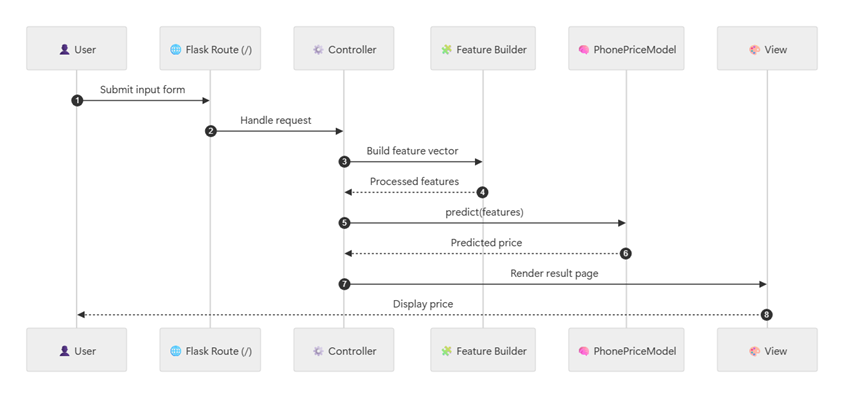
\includegraphics[width=0.92\textwidth]{graphics/price_prediction_flow.png}
    \caption{Luồng nghiệp vụ dự đoán giá điện thoại}
    \label{fig:price-prediction-flow}
\end{figure}

Luồng nghiệp vụ thứ hai là quản lý mô hình dành cho data scientist. Từ dashboard \texttt{/data-science}, có thể xem thống kê dữ liệu, nhập thêm bản ghi thủ công hoặc CSV, sinh dữ liệu tổng hợp, khởi tạo huấn luyện với siêu tham số mới, so sánh các version, đổi active model hoặc xóa một version không còn dùng. Toàn bộ phần này được nối về lớp mô hình trung tâm để giữ cho pipeline huấn luyện và pipeline suy luận vẫn dùng chung logic dữ liệu.

\begin{figure}[H]
    \centering
    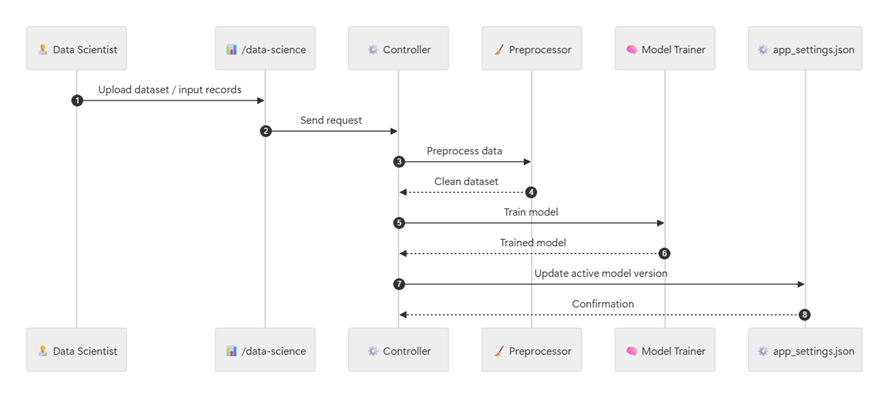
\includegraphics[width=0.92\textwidth]{code/ml_flow.png}
    \caption{Luồng nghiệp vụ quản lý và huấn luyện mô hình}
    \label{fig:ml-flow}
\end{figure}

Luồng nghiệp vụ thứ ba là quản lý người dùng dành cho admin. Tại \texttt{/admin}, phần quản trị tài khoản được giữ tách biệt với dữ liệu và mô hình. Admin có thể thêm, sửa, xóa người dùng, nhưng không trực tiếp thao tác với artifact học máy. Cách tách vai trò này giữ cho phần quản trị tài khoản không lẫn với phần vận hành machine learning.

\begin{figure}[H]
    \centering
    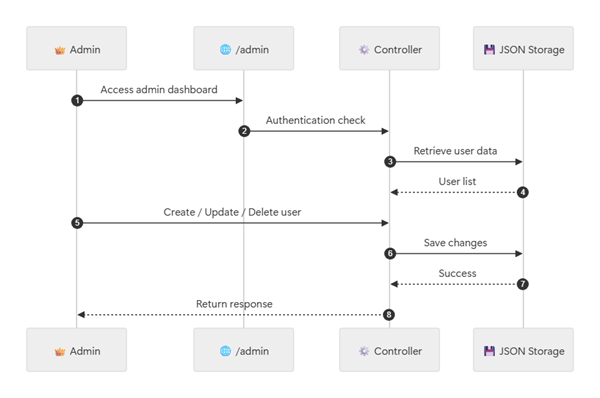
\includegraphics[width=0.92\textwidth]{code/admin_flow.png}
    \caption{Luồng nghiệp vụ quản trị người dùng của admin}
    \label{fig:admin-flow}
\end{figure}

\subsection{Các công nghệ triển khai chính}

Stack công nghệ của hệ thống được lựa chọn theo định hướng nhất quán và phù hợp với phạm vi triển khai của đề tài. Mỗi công nghệ trong stack đảm nhiệm một vai trò riêng trong quá trình xây dựng, huấn luyện, vận hành và đánh giá hệ thống.

\noindent\textasteriskcentered\ \textbf{Flask}

\begin{center}

\includegraphics[width=6cm]{graphics/tech_stack/flask.png}
\end{center}

\texttt{Flask} là web framework trung tâm của hệ thống, phù hợp với các ứng dụng cần cấu trúc gọn, linh hoạt và dễ kiểm soát luồng xử lý. Với đặc điểm nhẹ nhưng mở rộng tốt, Flask đóng vai trò kết nối giữa giao diện, logic nghiệp vụ và mô hình học máy trong cùng một ứng dụng.

Ứng dụng trong hệ thống:
\begin{itemize}
    \item Tạo web app trung tâm cho toàn bộ hệ thống dự đoán giá điện thoại.
    \item Định nghĩa các route chính như \texttt{/}, \texttt{/login}, \texttt{/admin} và \texttt{/data-science}.
    \item Quản lý session đăng nhập, điều hướng theo vai trò người dùng và cơ chế \texttt{flash} để phản hồi thao tác.
    \item Render giao diện HTML server-side cho guest, admin và data scientist.
\end{itemize}

\noindent\textasteriskcentered\ \textbf{Python}

\begin{center}

\includegraphics[width=4cm]{graphics/tech_stack/python.png}
\end{center}

\texttt{Python} là ngôn ngữ triển khai thống nhất của toàn bộ hệ thống. Điểm mạnh của Python nằm ở cú pháp dễ đọc, hệ sinh thái thư viện rộng và khả năng kết nối mượt giữa lập trình web, xử lý dữ liệu và học máy.

Ứng dụng trong hệ thống:
\begin{itemize}
    \item Triển khai toàn bộ backend, controller logic và dữ liệu runtime của ứng dụng.
    \item Bao phủ các bước xử lý dữ liệu, huấn luyện mô hình, versioning và suy luận.
    \item Cho phép kết nối liền mạch giữa Flask, pandas, scikit-learn, joblib và các thư viện trực quan hóa.
\end{itemize}

\noindent\textasteriskcentered\ \textbf{scikit-learn}

\begin{center}

\includegraphics[width=6cm]{graphics/tech_stack/scikit_learn.png}
\end{center}

\texttt{scikit-learn} là thư viện học máy trung tâm trong hệ thống, cung cấp đầy đủ các thành phần để xây dựng pipeline huấn luyện và suy luận. Trong đề tài này, thư viện được dùng như lõi triển khai cho mô hình hồi quy Random Forest và cho các bước tiền xử lý đặc trưng.

Ứng dụng trong hệ thống:
\begin{itemize}
    \item Cung cấp \texttt{RandomForestRegressor} cho bài toán dự đoán giá.
    \item Cung cấp \texttt{ColumnTransformer}, \texttt{SimpleImputer}, \texttt{OneHotEncoder} và \texttt{Pipeline} để xây dựng pipeline tiền xử lý và huấn luyện nhất quán.
    \item Hỗ trợ \texttt{train\_test\_split} và các metric đánh giá như MAE, RMSE và $R^2$.
    \item Cho phép tái sử dụng cùng một logic dữ liệu giữa pha training và pha inference.
\end{itemize}

\noindent\textasteriskcentered\ \textbf{pandas và NumPy}

\begin{center}

\includegraphics[width=6cm]{graphics/tech_stack/pandas_numpy.png}
\end{center}

\texttt{pandas} là thư viện xử lý dữ liệu bảng, còn \texttt{NumPy} cung cấp nền tảng tính toán số hiệu năng cao. Hai thư viện này thường đi cùng nhau trong các hệ thống machine learning, phụ trách tổ chức dữ liệu dạng bảng và hỗ trợ các phép toán số, biến đổi mảng dữ liệu.

Ứng dụng trong hệ thống:
\begin{itemize}
    \item Đọc, hợp nhất, chuẩn hóa và ghi dữ liệu huấn luyện từ các tệp CSV.
    \item Hỗ trợ nhập bản ghi thủ công và import dữ liệu hàng loạt từ dashboard quản trị dữ liệu.
    \item Thực hiện các phép biến đổi đặc trưng, thao tác số và chuẩn bị dữ liệu đầu vào cho pipeline học máy.
    \item Hỗ trợ xử lý dữ liệu batch trong các tình huống mở rộng hoặc tiền xử lý phân tích.
\end{itemize}

\noindent\textasteriskcentered\ \textbf{SciPy}

\begin{center}

\includegraphics[width=5cm]{graphics/tech_stack/scipy.png}
\end{center}

\texttt{SciPy} là thư viện bổ trợ cho hệ sinh thái tính toán khoa học trong Python. Dù không phải thành phần trung tâm của lớp web, thư viện này hỗ trợ môi trường phân tích dữ liệu và các tác vụ tính toán đi kèm khi hệ thống cần mở rộng sang các thao tác số sâu hơn.

Ứng dụng trong hệ thống:
\begin{itemize}
    \item Bổ sung cho lớp tính toán số và các thao tác phân tích dữ liệu phụ trợ.
    \item Tạo nền tảng mở rộng cho các xử lý định lượng hoặc thống kê trong các bước EDA và thực nghiệm.
\end{itemize}

\noindent\textasteriskcentered\ \textbf{joblib}

\begin{center}

\includegraphics[width=3cm]{graphics/tech_stack/joblib.png}
\end{center}

\texttt{joblib} là thư viện chuyên dùng cho việc tuần tự hóa và nạp lại các đối tượng Python có kích thước lớn, đặc biệt phù hợp với các artifact học máy. Trong hệ thống này, joblib đóng vai trò quan trọng ở lớp persistence của mô hình.

Ứng dụng trong hệ thống:
\begin{itemize}
    \item Lưu và nạp lại các model version dưới dạng \texttt{model.pkl}.
    \item Hỗ trợ cơ chế quản lý version mô hình theo từng thư mục artifact riêng biệt.
    \item Giúp thời gian nạp mô hình cho suy luận runtime nhanh và ổn định hơn.
\end{itemize}

\noindent\textasteriskcentered\ \textbf{kagglehub}

\begin{center}

\includegraphics[width=8cm]{graphics/tech_stack/kagglehub.png}
\end{center}

\texttt{kagglehub} là thành phần phục vụ bước thu nhận dữ liệu nguồn từ Kaggle. Công cụ này hỗ trợ chuẩn hóa bước thu nhận dữ liệu, nhờ đó giảm phụ thuộc vào thao tác thủ công và nâng cao tính tái lập khi huấn luyện lại mô hình.

Ứng dụng trong hệ thống:
\begin{itemize}
    \item Tải dataset từ tham chiếu Kaggle đã được cấu hình sẵn.
    \item Chuẩn hóa bước thu nhận dữ liệu đầu vào để thuận tiện cho việc tái sử dụng và huấn luyện lại.
\end{itemize}

\noindent\textasteriskcentered\ \textbf{Matplotlib và Seaborn}

\vspace{0.5\baselineskip}
\begin{center}

\includegraphics[width=8cm]{graphics/tech_stack/matplotlib_seaborn.jpg}
\end{center}

\texttt{Matplotlib} là thư viện trực quan hóa nền tảng, còn \texttt{Seaborn} mở rộng thêm lớp trực quan hóa thống kê với phong cách biểu đồ phù hợp cho phân tích dữ liệu. Hai công nghệ này được sử dụng chủ yếu ở pha EDA, phân tích chất lượng dữ liệu và sinh hình phục vụ báo cáo.

Ứng dụng trong hệ thống:
\begin{itemize}
    \item Tạo các biểu đồ phân phối, quan hệ đặc trưng và trực quan hóa dữ liệu trước huấn luyện.
    \item Sinh các artifact hình ảnh dùng trong báo cáo, dashboard phân tích và phần giải thích dữ liệu.
    \item Hỗ trợ data scientist quan sát dữ liệu và đọc hành vi của tập huấn luyện theo hướng trực quan hơn.
\end{itemize}

\noindent\textasteriskcentered\ \textbf{Lưu trữ cục bộ}

Lưu trữ cục bộ là tầng storage hiện tại của hệ thống trong phạm vi đề tài. Thay vì sử dụng cơ sở dữ liệu quan hệ hay object storage từ đầu, hệ thống dùng các tệp CSV, JSON và thư mục artifact version để giữ cấu trúc vận hành đơn giản, dễ quan sát và dễ phục hồi.

Ứng dụng trong hệ thống:
\begin{itemize}
    \item Lưu dữ liệu huấn luyện cục bộ dưới dạng CSV.
    \item Lưu trạng thái vận hành, tài khoản và active model dưới dạng JSON.
    \item Lưu các artifact mô hình theo từng thư mục version để thuận tiện cho việc rollback, so sánh và kích hoạt mô hình.
\end{itemize}
